\documentclass[twocolumn]{article}

\usepackage{amsmath}
\usepackage{caption}
\usepackage{graphicx}
\usepackage{float}

% Make table names in captions boldfaced
\captionsetup[table]{labelfont=bf}
\captionsetup[figure]{labelfont=bf}

\begin{document}
	
\title{Measuring the Speed of Light Using the Fizeau-Foucault Method}
\author{Robert Gregory, Raymond Jang, Jack Nelson}
\date{October 2016}

 % hacky trick to get a one-column abstract in a two-column article
\maketitle
\begin{abstract}
	Determining the value of nature's fundamental constants has been a basic function of physics since the founding of modern science.
	In this paper, we report our efforts to measure the speed of light in air to within ten percent of the accepted modern definition of 299,792 km/sec using a modernized version of the Foucault-Fizeau technique.
	Our measured value of $299,000 km/sec \pm 4\%$ shows that the speed of light can be accurately measured using this technique to within even 5\%.
\end{abstract}	
\section{Introduction}
	\label{sec:Intro}
	Our objective was to experimentally measure the speed of light $c_m$ in air using the Foucault method. 
	The paper is structured as follows:
	
	\S\ref{sec:Intro} provides an overview of the measurement of the speed of light, starting with a summary of historical attempts dating back to the 17th century.
	An overview of our particular technique of measurement is given, as well as a derivation of the equation used to calculate the speed of light from the quantities directly measured in our method.
	\S\ref{sec:Methods} describes the detailed experimental technique used to arrive at our measurement, as well as a discussion of potential sources of error, and ways we attempted to eliminate error, both random and systematic.
	\S\ref{sec:Results} presents the results of our experiment, including a full description of all calculations made, as well as our error analysis.
	\S\ref{sec:Conclusion} summarizes our experiment and findings.
		
	\subsection{Historical Background}
	
		The finite nature of light's speed has been questioned for centuries. 
		Most studies of the speed of light measure the time required for the light to travel a given distance. 
		Because of the apparent instantaneity of its travel in most human-scale settings, it wasn’t until scientific techniques and instruments matured in the late 17th and early 18th centuries that the nature of the speed of light could truly be investigated. 
		
		In 1638, the famed Renaissance scientist Galileo Galilei theorized about the nature of light's travel in the form of a fictional conversation between three Italians, Salviati, Sagredo, and Simplicio in his treatise \textit{Dialogues Concerning Two New Sciences}.\cite{galilei_dialogues_1638}
		In the treatise, the three Italians speculate whether the speed of light is finite or infinite, and conclude that, if it is finite, it must be of very great magnitude:
		
		\begin{quotation}
			\noindent
			\textit{\textbf{Sagredo}} \newline 
			\textit{But of what kind and how great must we consider this speed of light to be? 
			Is it instantaneous or momentary or does it like other motions require time? 
			Can we not decide this by experiment?}
			
			\noindent \newline
			\textit{\textbf{Simplicio}} \newline 
			\textit{Everyday experience shows that the propagation of light is instantaneous; for when we see a piece of artillery fired, at great distance, the flash reaches our eyes without lapse of time; but the sound reaches the ear only after a noticeable interval.}
			
			
			\noindent \newline
			\textit{\textbf{Salviati}} \newline
			\textit{The small conclusiveness of these and other similar observations once led me to
			devise a method by which one might accurately ascertain whether illumination, i.e., the propagation of light, is really instantaneous. The fact that the speed of sound is as high as it is, assures us that the motion of light cannot fail to be extraordinarily swift.}
		\end{quotation}
		
		Galileo, through Salviati, goes on to explain his design of an experiment to determine whether light's rate of travel is finite or instantaneous using two persons equipped with lanterns they can quickly cover and uncover separated by a distance of a few miles . 
		The idea, then, is that as soon as one person covers their lantern, the second person covers theirs. 
		If the first person sees any delay in the covering of the second's lantern, they can conclude that light's speed is finite. 
		On the other hand, if the first person detects no delay in the covering of the second's lantern, they can conclude that light is instantaneous.
		
		Of course, at the distances which Salviati proposes, the speed of light is much too large to be detected by human reflexes. 
		Salviati (Galileo) admits that his own attempt at the experiment was inconclusive:
		
		\begin{quotation}
			\noindent
			\textit{\textbf{Sagredo}} \newline
			\textit{This experiment strikes me as a clever and reliable invention. 
			But tell us what you conclude from the results.}
			
			\noindent \newline
			\textit{\textbf{Salviati}} \newline
			\textit{In fact I have tried the experiment only at a short distance, less than a mile, from
			which I have not been able to ascertain with certainty whether the appearance of the opposite light was instantaneous or not; but if not instantaneous it is extraordinarily rapid.}
		\end{quotation}
		
		Despite the flawed nature of Galileo's proposed experiment, he did identify the importance of having a long baseline distance to making an accurate measurement of the speed of light, if it was indeed finite.
		
		In the subsequent centuries following Galileo's inconclusive theorizing on light, several scientists made the case that light's travel was indeed finite. 
		In 1676, Danish astronomer Ole R\o{}mer used the timing of the eclipses of Jupiter's moon Io, appropriately discovered by Galileo in 1610, to demonstrate that light's speed was finite.\cite{romer_motion_1677}
		
		Astronomer Christian Huygens, R\o{}mer's contemporary, readily accepted R\o{}mer's findings, and used his observations to estimate the speed of light to be equivalent to 230,000 km/s, about 25\% less than the current accepted value.
		This marked the first numerical value for the speed of light given by a scientist.\cite{bobis_cassini_2008}
		
		A quarter century later in 1704, Isaac Newton wrote about R\o{}mer's findings in \textit{Opticks} and estimated it would take light ``seven or eight minutes" to travel from the Sun to the Earth.\cite{newton_opticks_1704} 
		In a 1729 letter to Edmond Halley published by the Royal Society of London, James Bradley reported the phenomenon of stellar aberration and estimated the Sun-Earth light travel time to be 8 minutes and 12 seconds, just seven seconds less than the modern accepted value of 8 minutes and 19 seconds.\cite{bradley_account_1729}
		
		\begin{table*}[!ht]
			\centering
			\begin{tabular}{c|llll}
				Year & Scientist(s)                 	& Method				& Value (km/sec)      & Percent Error \\ \hline
				1638 & Galileo Galilei              	& Covered Lanterns		& Inconclusive 		  & N/A           \\
				1676 & Ole R\o{}mer, Christian Huygens 	& Eclipse of Io			& 230,000 			  & 25\%          \\
				1729 & James Bradley					& Aberration of Light	& 301,000			  & 0.4\%		\\
				1849 & Hippolyte Fizeau             	& Toothed Wheel			& 315,000 			  & 5\%           \\
				1862 & Leon Foucault                	& Rotating Mirror		& 298,000 			  & 0.6\%         \\
				1878 & Albert Michelson             	& Rotating Mirror, 600m Baseline	& 299,910 & 0.04\%        \\
				1926 & Albert Michelson            		& Rotating Mirror, 35km Baseline		 & 299,798 & 0.001\%  \\
				1983 & Bureau International des Poids Mesures	& Standard Definition	& 299,792.458	& Exact   
			\end{tabular}
			\caption{\textbf{Measurements of the speed of light since the 17th century}}
			\label{tab:HistoricalMasurements}
		\end{table*}
		
		The first terrestrial scientific attempts to systematically measure the speed of light were made at first cooperatively, and then separately, by Hippolyte Fizeau and L\'{e}on Foucault starting around 1845.\cite{sanders_velocity_1965}
		Fizeau used a rotating toothed wheel to modulate a light source across a distance of 8km to a fixed mirror which reflected the light back to the cog wheel. 
		Fizeau increased the speed of the wheel until light from one notch in the wheel was blocked by the subsequent tooth on its return trip. With this technique, Fizeau calculated the speed of light to be 315,000km/sec, about 5\% higher than the modern value.\cite{sanders_velocity_1965}
		
		Charles Wheatstone in 1834 proposed using a rotating mirror rather than a cog wheel and measuring the returning light's displacement when reflected off the rotating mirror at high angular velocities. 
		This technique was more fully developed by Foucault starting in 1850, and in 1862 Foucault measured a value of 298,000km/sec using a baseline of only 20m.\cite{sanders_velocity_1965}
		
		Foucault's method was further refined and expanded by Albert Abraham Michelson in 1878 using a baseline of 600m, obtaining a result of 299,910km/sec.\cite{michelson_experimental_1878}
		Nearly fifty years later in 1926, Michelson attempted a more accurate measurement, this time using a precisely-measured baseline of 35km between Mount Wilson and Mount San Antonio near Pasadena, California.
		The refined experiment measured a value of 299,798$\pm$4 km/sec, which is within 0.001\% error of the modern value of 299,792 km/s.\cite{michelson_measurement_1927}
		
		Table \ref{tab:HistoricalMasurements} summarizes the historical measurements of the speed of light since the 17th century up to the modern standard definition by the Bureau International des Poids et Mesures in 1983.\cite{_bipm_1984}
		
		
	\subsection{Theory of Experiment}
		Our experimental technique is heavily based on the direct-measurement technique Fizeau and Foucault pioneered in the mid-19th century.
		The central apparatus of the experiment is a two-sided variable-speed rotating mirror powered by a DC electric motor.
		A monochromatic red laser is focused onto the mirror while it rotates at angular speeds of up to 1,500Hz.
		A slightly concave fixed mirror is located approximately 6m away at angle $\theta$ relative to the incident laser path such that as the rotating mirror sweeps through angle $\theta$, it reflects laser light onto the fixed mirror.
		The concave fixed mirror then reflects the laser light and focuses it back onto the rotating mirror.
		
		\begin{figure}[!ht]
			\centering
			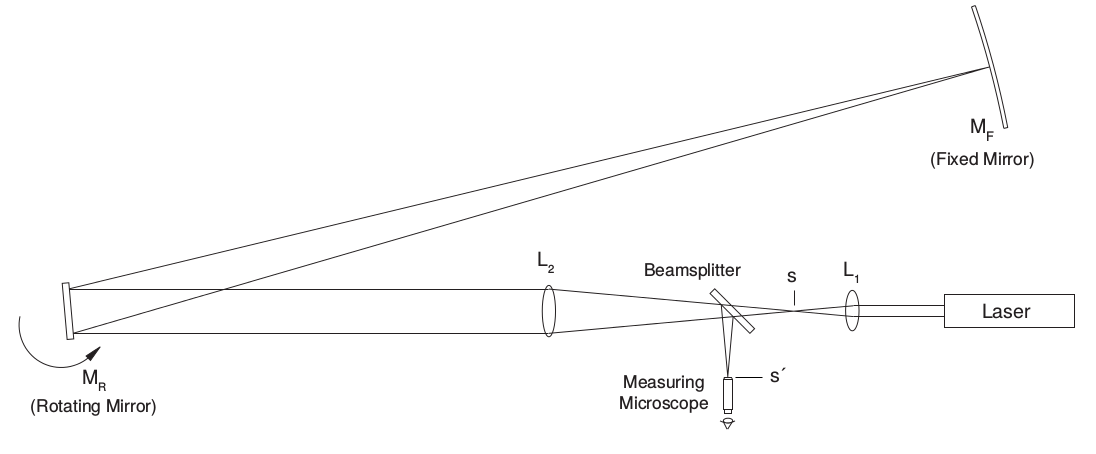
\includegraphics[width=0.49\textwidth]{Images/FoucaultMethodDiagram.png}
			\caption{\textbf{Configuration of a Fizeau-Foucault method of measuring the speed of light using a rotating mirror. Figure 1 of \cite{lee_instruction_????}. \copyright PASCO Scientific.}}
			\label{fig:FoucaultDiagram}
		\end{figure}
		
		If the speed of light were infinite and the travel time between the rotating and fixed mirrors instantaneous, the mirror would not rotate during the light's travel between the mirrors, and so the light would be reflected back towards the laser source at exactly the same angle it had entered.
		
		However, if the speed of light is finite, there should be a time-of-flight delay as the light travels from the rotating mirror to the fixed mirror and back.
		During this time, the rotating mirror should rotate an angular distance $\theta_s$, such that the angle of incidence of the light as it returns is slightly different from the angle of incidence of when it was initially reflected.
		This results in the returning light being slightly deflected from its original path incident to the rotating mirror.
		
		If we place a half-silvered beam splitter in between the laser source and the rotating mirror such that light from the rotating mirror is partially reflected into a microscope, we can measure the minute deflection of the laser light due to the rotating mirror's motion during the light's time-of-flight delay.
		
		The experimental configuration is shown in Figure \ref{fig:FoucaultDiagram}.
		
\section{Methods and Procedures}
	\label{sec:Methods}
	\subsection{Method Description}
		Our measurements were made using the PASCO OS-9261 Speed of Light Apparatus Kit by PASCO Scientific.
		The kit included the components shown in Figure \ref{fig:LabEquip}.
		\begin{figure}[!ht]
			\centering
			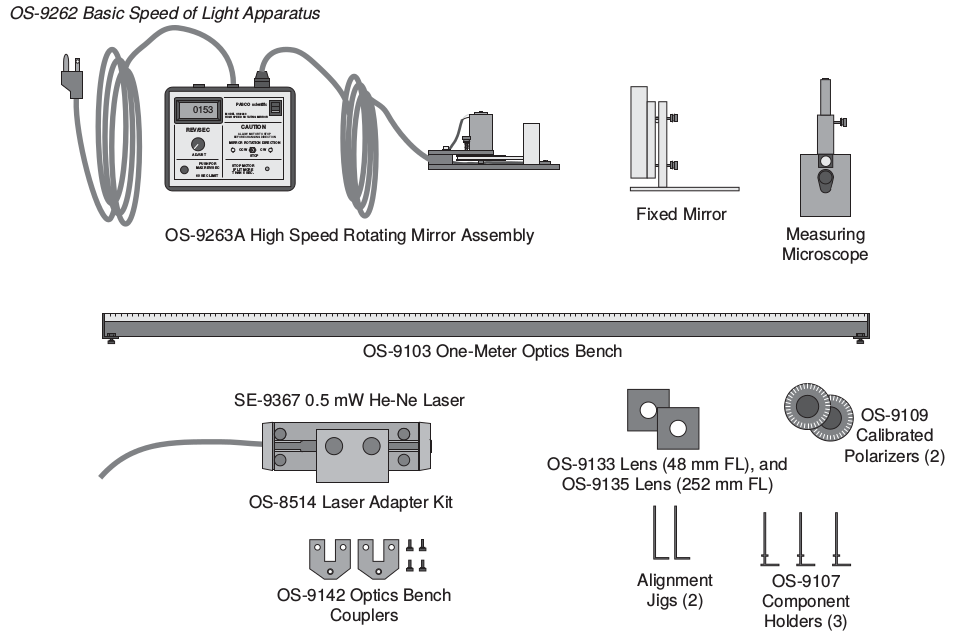
\includegraphics[width=0.49\textwidth]{Images/PASCO_Equipment.png}
			\caption{\textbf{PASCO OS-9261 Speed of Light Apparatus Kit. Figure 4 in \cite{lee_instruction_????}. \copyright PASCO Scientific.}}
			\label{fig:LabEquip}
		\end{figure}
		The Optics Bench was first placed on a flat level surface and loosely attached to the Laser Alignment Bench.  
		We then joined the two benches together using Bench Couplers with leveling screws that were set at an equal height.  
		The Rotating Mirror Assembly was then placed on the Optics Bench so that the edge of the rotating mirror was aligned with the 17cm mark of the Optics Bench ruler.
		
		First, Lens 1 ($L_1$) was mounted on a Component Holder and placed at the $93.0 cm$ mark of the Optics Bench, then adjusted slightly along the bench until it focused the laser onto the center of $M_r$. 
		Lens 2 ($L_2$) was between $L_1$ and $M_r$ then placed near the $62.2 cm$ mark on the optics bench and also adjusted until the beam was focused on $M_r$.  
		The beam splitter and measuring microscope were then placed between $L_1$ and $L_2$ at $82.0 cm$ on the Optics Bench.  
		The beamsplitter adjustment lever on the microscope was positioned in the 45-degree downward orientation with respect to the incident laser beam so as to reflect the returning beam reflected by the $M_r$ upwards into the measuring microscope.
		
		The fixed spherical mirror $M_f$ was then placed $6.65m$ from $M_r$ at an angle of $\sim12^{\circ}$ from the path of the beam.
		The instruction manual provided by PASCO \cite{lee_instruction_????} recommended placing the fixed mirror at least $8m$ from the rotating mirror, however the space available in our lab limited us to less than $7m$.
		The optics bench configuration at this point is shown in Figure \ref{fig:EquipConfig}.
		\begin{figure}[!ht]
			\centering
			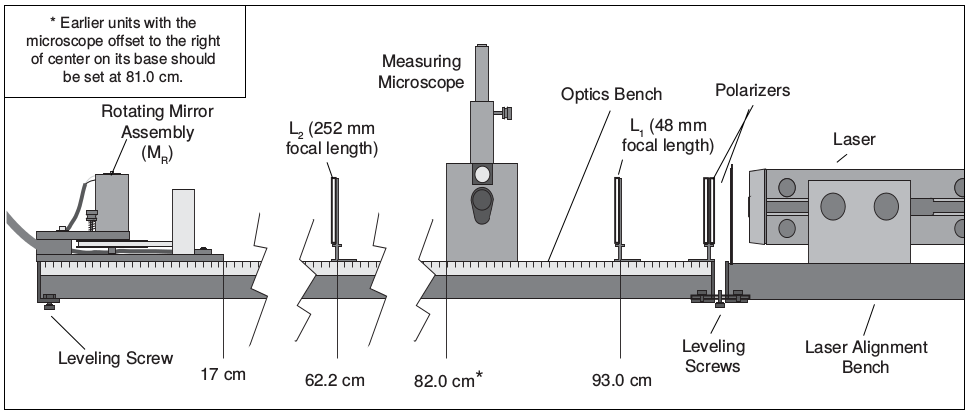
\includegraphics[width=0.49\textwidth]{Images/PASCO_EquipmentAlignment.png}
			\caption{\textbf{Configuration of the optics bench. Figure 5 in \cite{lee_instruction_????}. \copyright PASCO Scientific.}}
			\label{fig:EquipConfig}
		\end{figure}
		
		After setup of the optics bench is complete, we rotated $M_r$ until the reflected beam intersected the fixed mirror.
		Alignment screws on $M_f$ were then used to reflect the beam back onto $M_r$.
		The beam was then refocused by slightly adjusting the position of $L_2$ on the optics bench.  
		
		Finally, two polarizers were placed on the optics bench between the laser and $L_1$ to control the intensity of the laser and prevent eye damage when looking through the microscope.
		
		When the optics bench and mirrors are configured correctly, the beam will be reflected from $M_r$ to $M_f$, back to $M_r$, and then into the microscope such that a single point of light is visible in the microscope amidst a background of interference patterns from stray reflections in the optics.

		The position of this point of light was measured using a micrometer which controlled the microscope.
		Accurate measurements of the beam deflection at varying angular speeds of $M_r$ could then be made by positioning the microscope crosshairs over the light beam and reading the micrometer value.
		
		Each measurement of beam deflection began by measuring the image point location with $M_r$ rotating at $1,500Hz$ in the clockwise direction.
		The $M_r$ rotation was placed in the clockwise rotation and was adjusted and displayed using was then dial on the rotating mirror assembly. 
		The motion of $M_r$ was then reversed, and a second measurement was made at $1,500Hz$ in the counterclockwise direction.
		The total beam deflection was taken as the difference between these two measurements.
			
	\subsection{Derivation of the Speed of Light Equation}
	\label{subsec:Derivation}
	We start by considering a laser, a rotating mirror $M_r$, and a fixed mirror $M_f$ in the configuration shown in Figure \ref{fig:MrMfAngles}. 
	Suppose a photon is emitted from the laser and reflected off the rotating mirror to a point $S$ located on the fixed mirror in euclidean space. 
	If $M_r$ is at an angle $\theta$ from the plane of the incident laser beam, the incident light will be reflected onto $M_f$ at an angle of 2$\theta$ by Snell's law.
	
	\begin{figure}[!ht]
		\centering
		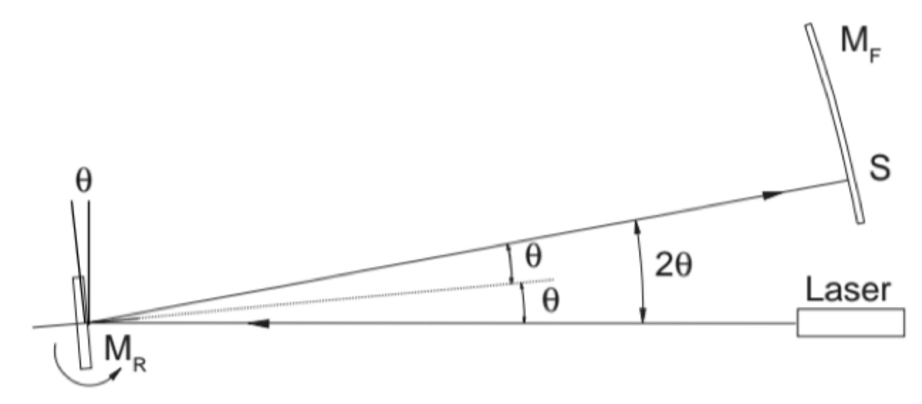
\includegraphics[width=0.49\textwidth]{Images/MrMfAngles.png}
		\caption{\textbf{Laser beam reflected an angle $2\theta$ by $M_r$ onto $M_f$ as image $S$.\cite{lee_instruction_????} \copyright PASCO Scientific}}
		\label{fig:MrMfAngles}
	\end{figure}
	Now suppose a second beam of light is emitted at a small time $\Delta t$ later. 
	The rotating mirror will have rotated by a total angle  $\theta + \Delta \theta$.
	Let the new image on $M_f$ be called $S_1$. 
	$S_1$ will be at an angle $2(\theta + \Delta \theta)$ from the plane of the laser by Snell's law again, as shown in Figure \ref{fig:MrMfAngles2}. 
	Call this quantity $\theta_1$:
	\begin{equation}
		\theta_1 = 2(\theta + \Delta \theta)
	\end{equation}
	\begin{figure}[!ht]
		\centering
		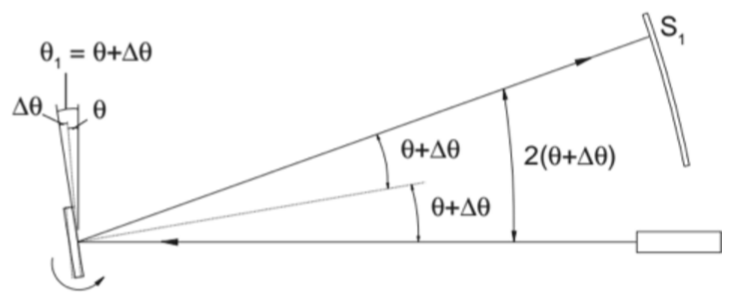
\includegraphics[width=0.49\textwidth]{Images/MrMfAngles2.png}
		\caption{\textbf{Image $S_1$ a small time $\Delta t$ later after $M_r$ rotates by angle $\Delta\theta$.\cite{lee_instruction_????} \copyright PASCO Scientific}}
		\label{fig:MrMfAngles2}
	\end{figure}
	
	Now let D be the distance between $M_r$ and $M_f$. 
	The distance between the original image $S$ and the second image $S_1$ formed at a small time $\Delta t$ later can be found from trigonometry. 
	Assuming both $S$ and $S_1$ lie on the arc of a circle of radius $D$, the arc length $\Delta S = S_1-S$ would be:
	\begin{equation*}
		\Delta S = S_1 - S = D(2\theta_1 - 2\theta)
	\end{equation*}
	\begin{equation*}
		= D[2(\theta + \Delta \theta) - 2\theta] = 2D\Delta\theta
	\end{equation*}
	\begin{equation}
		\Rightarrow \Delta S = 2D\Delta\theta
		\label{eq:DeltaS}
	\end{equation}
	
	Now suppose a beam splitter and a lens $L_2$ is placed between the laser and rotating mirror. 
	Constructing a virtual image of $M_r$, as shown in Figure \ref{fig:VirtualImage}, will allow the arc length $\Delta S$ as seen through lens $L_2$ to be computed. 
	\begin{figure}[!ht]
		\centering
		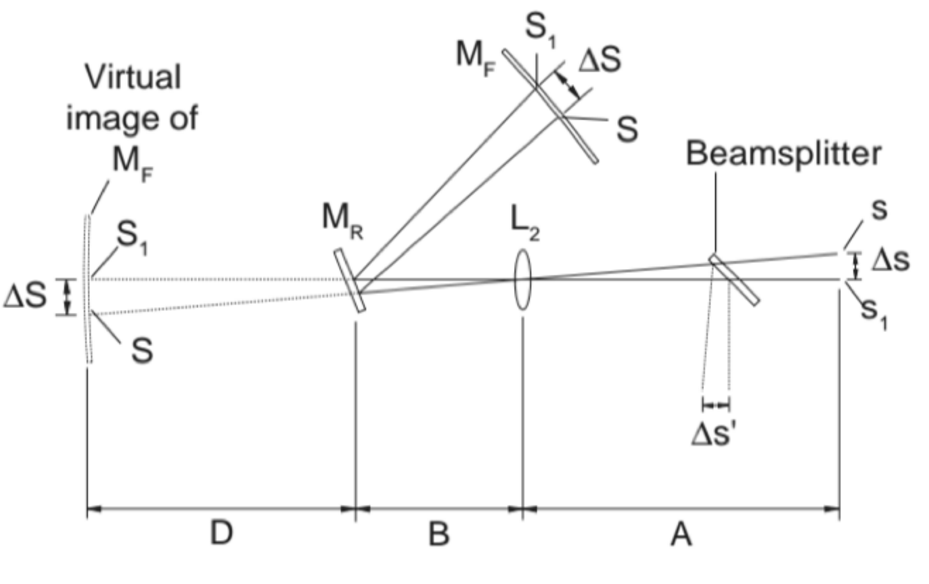
\includegraphics[width=0.49\textwidth]{Images/VirtualImageDiagram}]
		\caption{\textbf{$\Delta S$ projected onto the virtual image of $M_r$.\cite{lee_instruction_????} \copyright PASCO Scientific}}
		\label{fig:VirtualImage}
	\end{figure}
	
	Lenses $L_2$ will distort the arc length $\Delta S$ by $i/o$ where $i$ is $A$, the distance from $L_2$ to the image, and $o$ is the distance from $l_2$ to the object at $D + B$. 
	The length $\Delta S$ will therefore become a new contracted length we'll call  $\Delta s'$ when the light passes through lens $L_2$. 
	With this, $\Delta s'$ is equal to:
	\begin{equation}
		\Delta s' = \frac{i}{o} \Delta S = (\frac{A}{D+B})\Delta S
		\label{eq:DeltaSPrime}
	\end{equation}
	
	Additionally, from Equation (\ref{eq:DeltaS}), $\Delta S$ was found to be twice the product of the distance between mirrors D and a tiny angle $\Delta \theta$. Substituting this information from Equation (\ref{eq:DeltaS}) into Equation (\ref{eq:DeltaSPrime}) gives:
	\begin{equation}
		\Delta s' = (\frac{A}{D+B})2D\Delta\theta
		\label{eq:DeltaSPrime2}
	\end{equation}
	
	The small angle $\Delta \Theta$ is really just the rotation rate of the mirror in radians per second $\omega$ divided by the speed of the laser beam. 
	
	Here, it will be assumed the laser travels at the speed of light in a vacuum $c$.
	This assumption will be shown to be valid in our conclusion in section \ref{sec:Conclusion}.
	
	Therefore, $\Delta \Theta$ can be written in terms of the rotation rate of $M_r$:
	\begin{equation}
		\Delta\theta = 2D\frac{w}{c}
		\label{eq:DeltaTheta}
	\end{equation}
	
	By substituting Equation (\ref{eq:DeltaTheta}) into Equation (\ref{eq:DeltaSPrime2}), the reflected image can be rewritten as:
	\begin{equation}
		\Delta s' = \frac{4A\omega D^2}{c(D+B)}
		\label{eq:DeltaSPrime3}
	\end{equation}
	
	Equation (\ref{eq:DeltaSPrime3}) can be solved for c by taking the reciprocal, yielding the result:
	\begin{equation}
		c = \frac{4A\omega D^2}{\Delta s'(D+B)}
		\label{eq:SpeedOfLightRadians}
	\end{equation}
	
	Equation (\ref{eq:SpeedOfLightRadians}) relates the small arc length $\Delta S$, shrunk to a shorter length called $\Delta s'$ by a lens $L_2$, to the speed of light. 
	Even though this derivation assumed two light pulses at a small time $\Delta t$ from one another, the result is valid for a continuous beam of light as long as the rotation rate of $M_r$ is constant. 
	
	Equation (\ref{eq:SpeedOfLightRadians}) predicts that as the angular velocity $\omega$ of $M_r$ is increased, the displacement $\Delta s'$ will also increase. 
	Conversely, as $\omega$ decreases, the displacement as viewed from the lens $L_2$ will decrease converging to zero displacement and a still image when the rotating mirror is stationary. 
	
	To adjust Equation (\ref{eq:SpeedOfLightRadians}) to use angular velocity units of Hertz rather than radians per second, we simply multiply the equation by a conversion factor of $2\pi$.
	Furthermore, we can break down Equation (\ref{eq:SpeedOfLightRadians}) into the components we'll be directly measuring.
	Since we measure the total deflection of the laser beam from the maximum clockwise deflection to the maximum counterclockwise deflection, the total displacement $\Delta s'$ is given by:
	\begin{equation}
		\Delta s' = s'_{cw} - s'_{ccw}
	\end{equation} 
	The angular frequency $f$ we directly measure is then the difference between the angular frequency at $s'_{cw}$ and $s'_{ccw}$:
	\begin{equation}
		f = f_{cw} - f_{ccw}
	\end{equation}
	This notation assumes the convention that a clockwise rotation is positive, and a counterclockwise rotation is negative.
	
	Our final equation for the experimental speed of light is then:
	\begin{equation} \label{eq:SpeedofLightCalc1}
	c = \frac{ 8\pi AD^2 (f_{cw} + f_{ccw})}
	{ (D + B) (s'_{cw} - s'_{ccw})}
	\end{equation}
	
	The deflections $s'_{cw}$ and $s'_{ccw}$, and the angular frequencies $f_{cw}$ and $f_{ccw}$ at each deflection measurement are measured to calculate an experimental value of $c$. 
	
\section{Results}
	\label{sec:Results}


	\subsection{Data}
		% raw deflection measurements
		\begin{table*}[] 
			
			\centering
			
			\begin{tabular}{c|c c c c}
				Trial ID & \begin{tabular}[c]{@{}c@{}}CW Measurement \\ (mm) ($\pm0.01$)\end{tabular} & \begin{tabular}[c]{@{}c@{}}CW Speed \\ (Hz) ($\pm5$)\end{tabular} & \begin{tabular}[c]{@{}c@{}}CCW Measurement \\ (mm) ($\pm0.01$)\end{tabular} & \begin{tabular}[c]{@{}c@{}}CCW Speed \\ (Hz) ($\pm5$)\end{tabular} \\ \hline
				11       & 10.17                                                          & 1503                                                        & 9.77                                                            & -1460                                                        \\
				12       & 10.19                                                          & 1505                                                        & 9.77                                                            & -1464                                                        \\
				13       & 10.18                                                          & 1510                                                        & 9.78                                                            & -1461                                                        \\ 
				21       & 10.16                                                          & 1506                                                        & 9.78                                                            & -1462                                                        \\
				22       & 10.18                                                          & 1503                                                        & 9.83                                                            & -1463                                                        \\
				23       & 10.22                                                          & 1507                                                        & 9.86                                                            & -1460                                                        \\ 
				31       & 12.00                                                          & 1508                                                        & 11.62                                                           & -1465                                                        \\
				32       & 12.00                                                          & 1505                                                        & 11.58                                                           & -1456                                                        \\
				33       & 12.00                                                          & 1507                                                        & 11.62                                                           & -1468                                                        \\
				34       & 12.10                                                          & 1510                                                        & 11.62                                                           & -1466  \\                                                  
			\end{tabular}
			\caption{\textbf{Laser deflection data taken during three separate sessions. Positive rotation speeds correspond to clockwise rotation of the rotating mirror, and negative speeds correspond to counterclockwise speeds.}}
			\label{tab:rawmeasure}
		\end{table*}
		
		
		
	Three sets of data were taken spread across three measurement sessions on different dates. 
	Table \ref{tab:rawmeasure} shows the measurements taken in each of the three sessions.
	The data is indexed by a trial ID. 
	The session each measurement belongs to is indicated by the leading digit of the trial ID. 
	For example, measurement 23 is the third measurement taken in the second set of data.
	For each set, measurements were taken at angular velocities of $\pm$1500 Hz for the rotating mirror. 
	
	Other values necessary for the calculation of the speed of light included the distance A between $L_1$ and $L_2$, the distance $B$ between $L_2$ and the rotating mirror, and the baseline distance $D$ between the rotating mirror and the fixed mirror. Measurements of each of these distances were taken and reported in Table \ref{tab:distances}.
		
	% distance measurement data
	\begin{table}[t]
		\centering
		\begin{tabular}{c|c}
			Dimension	&	Measured Value	\\ \hline
			A	&	$0.260\pm0.007m$	\\
			B	&	$0.481\pm0.007m$	\\
			D	&	$6.65\pm0.01m$	\\
		\end{tabular}
		\caption{\textbf{Measurements of the lengths $A$, $B$, and $D$.}}
		\label{tab:distances}
	\end{table}
	
	
	\subsection{Calculations} \label{subsec:Calculations}
	The equation relating the dimensional measurements $A$, $B$, and $C$, as well as the deflection $\Delta s' = s'_{cw} - s'_{ccw}$ and angular frequency  and $f = f_{cw} -f_{ccw}$, was derived in section \ref{subsec:Derivation} as Equation (\ref{eq:SpeedofLightCalc1}), and restated below as Equation (\ref{eq:speedoflight_calcs}):
	
	\begin{equation} \label{eq:speedoflight_calcs}
	c = \frac{ 8\pi AD^2 (f_{cw} - f_{ccw})}
	{ (D + B) (s'_{cw} - s'_{ccw})}
	\end{equation}
	
	Table \ref{tab:deflection} shows $\Delta s'$ and $f$ for each measurement in mm and Hertz, respectively.
	$\Delta s'$ was obtained by taking the difference between the clockwise deflection measurement $s'_{cw}$ and the counterclockwise deflection measurement $s'_{ccw}$.
	Similarly, $f$ was obtained by taking the difference between the frequency $f_{cw}$ at which the clockwise measurement was made, and the frequency $f_{ccw}$ at which the counterclockwise measurement was made.
	
	% deflection data TODO - Might be redundant
	\begin{table}[t]
		\centering
		\begin{tabular}{l|l l}
			
			Trial ID & \begin{tabular}[c]{@{}l@{}}Deflection $\Delta s'$\\ (mm)($\pm0.035$)\end{tabular} &  \begin{tabular}[c]{@{}l@{}}Angular Frequency $f$\\ (Hz)($\pm7$)\end{tabular} \\ \hline
			11       & 0.40	&	2963       \\
			12       & 0.45	&	2969       \\
			13       & 0.40 &	2971      \\
			21       & 0.40 &	2968      \\
			22       & 0.35 &	2966      \\
			23       & 0.36 &	2967      \\
			31       & 0.38 &	2973      \\
			32       & 0.42 &	2961      \\
			33       & 0.38 &	2975      \\
			34       & 0.48 &	2976      \\  \hline
			Average	 & $0.40\pm0.01mm$ &	$2969\pm2Hz$                                            
		\end{tabular}%
		\caption{\textbf{Laser deflection and mirror rotational frequency for each trial with associated measurement error. Average values across all trials are provided in the bottom row, along with their associated standard error uncertainties}}
		\label{tab:deflection}
	\end{table}
	
	$\Delta s'$ and $f$ were averaged across all the measurements to obtain a best value for each.
	The best values for the deflection and mirror angular frequency are shown in the bottom row of table \ref{tab:deflection}.
	
	% mean measurements data TODO - Possible redundant
	\iffalse
	\begin{table*}[t]	
		\centering
		\begin{tabular}{c|c c c}
			
		    Data Set	& \begin{tabular}[c]{@{}c@{}}Measurement Mean, CW\\ (mm)\end{tabular} & \begin{tabular}[c]{@{}c@{}}Measurement Mean, CCW\\ (mm)\end{tabular} & \begin{tabular}[c]{@{}c@{}}Mean Deflection\\ (mm)\end{tabular} \\ \hline
			Set 1 & 10.18                                                               & 9.27                                                                 & 0.91                  \\
			Set 2 & 10.18                                                               & 9.32                                                                 & 0.86                                                   \\
			Set 3 & 12.02                                                               & 11.11                                                                & 0.92                                        \\       
		\end{tabular}
		\caption{\textbf{Mean measurements for each set of data averaged with respect to mirror rotation speed and direction.}}
		\label{tab:meanvalues}
	\end{table*}
	\fi
	
	\iffalse
	\begin{table*}[t]
		\centering
		\begin{tabular}{c|l l l l l}
			
			Data Set	& $\Delta s'$ (mm) & $f$ (Hz) & A (m) & B (m)& D (m)\\ \hline
			Set 1 & 0.42$\pm0.02$                                                               & 2968$\pm4$                                                                & 0.260$\pm0.001$	& 0.481$\pm0.001$	& 6.65$\pm0.01$                 \\
			Set 2 & 0.37$\pm0.06$                                                               &  2967$\pm3$  &  0.260$\pm0.001$ & 0.481$\pm0.001$ & 6.65 $\pm0.01$                                   \\
			Set 3 & 0.41$\pm0.05$                                                               & 2971$\pm6$                                                               & 0.326$\pm0.001$ & 0.45$\pm0.001mm$ & 0.01$\pm0.01Hz$                                        \\       
		\end{tabular}
		\caption{\textbf{All measured values for each set with their associated uncertainties.}}
		\label{tab:meanvalues}
	\end{table*}
	\fi
	% average rotation speed data
	\iffalse
	\begin{table*}[t]
		\centering
		\begin{tabular}{c|c c c}
			
			 Data Set & \begin{tabular}[c]{@{}c@{}}Mean CW Rotation Speed \\ (Hz)($\pm$5)\end{tabular} & \begin{tabular}[c]{@{}c@{}}Mean CCW Rotation Speed \\ (Hz)($\pm$5)\end{tabular} & \begin{tabular}[c]{@{}c@{}}Mean Deflection Frequency \\ (Hz)($\pm$10)\end{tabular} \\ \hline
			Set 1 & 1506                                                                            & -1461                                                                             & 2967                                                                               \\
			Set 2 & 1505                                                                            & -1462                                                                             & 2967                                                                               \\
			Set 3 & 1508                                                                            & -1464                                                                             & 2971  \\                                                                      
		\end{tabular}
		\caption{\textbf{Mean measurement rotation speeds for each set of data.}}
		\label{tab:averagerotf}
	\end{table*}
	\fi
	% speed of light
	\iffalse
	\begin{table*}[!ht]
		\centering
		\begin{tabular}{c|c c c c}
			Data Set  & \begin{tabular}[c]{@{}c@{}}$c$ \\ ($km/sec$)\end{tabular} & \begin{tabular}[c]{@{}c@{}}Random Uncertainty \\ ($\pm km/sec$)\end{tabular} & \begin{tabular}[c]{@{}c@{}}Systematic Uncertainty \\ ($\pm km/sec$)\end{tabular} & \begin{tabular}[c]{@{}c@{}}Total Uncertainty \\ ($\pm km/sec$)\end{tabular} \\ \hline
			Set 1 & $290,000$                                           & 20,000 &    30,000        & 30,000                                                  \\
			Set 2 & $330,000$                                           & 50,000	&  30,000   & 60,000                \\     
			Set 3 & $310,000$	&	40,000	&	30,000	&	50,000	\\                              
		\end{tabular}
		\caption{\textbf{Calculated values of the speed of light}}
		\label{tab:cvals}
	\end{table*}
	\fi
	We arrive at our measured value for the speed of light $c_m$ by substituting the measured quantities $A$, $B$, and $D$ given in table \ref{tab:distances}, and the mean deflection $\Delta s'_\mu$ and angular frequency $f_\mu$ given in table \ref{tab:deflection} into Equation (\ref{eq:speedoflight_calcs}) and solving:
	\begin{equation}
		c_{m} = \frac{8\pi AD^2 f_\mu}{(D+B)\Delta s'_\mu}
	\end{equation}
	\begin{equation}
		c_{m} = \frac{(0.260m)(6.65m)^2(2969Hz)}{(6.65m + 0.481m)(0.40\times 10^{-3}m)}
	\end{equation}
	
	Our final value for $c_m$ is given in Equation (\ref{eq:MeasuredSpeedofLight}) and reported with random and systematic uncertainties $\delta c_{ran}$ and $\delta c_{sys}$.
	These uncertainties will be explained and calculated in section \ref{subsec:error}.
	\begin{equation*}
	c_m = c_{best}\pm \delta c_{ran} \pm \delta c_{sys}
	\end{equation*}
	\begin{equation}
		\label{eq:MeasuredSpeedofLight}
		c_{m} = 299,000\pm 9,000\pm 9,000 km/sec
	\end{equation}
	
	We can additionally report $c_m$ with a measure of total uncertainty and total percent error as well:
	\begin{equation*}
		c_m = 299,000\pm 13,000 km/sec = 
	\end{equation*}
	\begin{equation}
		= 299,000km/sec\pm 4\%
	\end{equation}
	
	The calculation of total uncertainty will be covered in section \ref{subsubsec:TotalError}.
	
	\subsection{Error Analysis} \label{subsec:error}
	We quantified both systematic and random uncertainty in our measurement.
	Section \ref{subsubsec:SystematicError} explains the calculation of the systematic uncertainty in our measurement, while section \ref{subsubsec:RandomError} shows our process of calculating the random uncertainty.
	
	The random and systematic uncertainties are also combined into a total measure of uncertainty by adding them in quadrature, although evaluating them separately gives more insight into the source of error in our measurements.
	
	\subsubsection{Systematic Error} \label{subsubsec:SystematicError}
		We first account for the experimental systematic error.
		In our equation for the speed of light given by Equation (\ref{eq:speedoflight_calcs}), we have five measured quantities, each of which have an associated systematic error: $A, B, D, \Delta s'$, and $f$.
		The relative importance of each contribution to uncertainty will be considered and the fractional systematic uncertainty for $c_m$ will be found by directly summing all five fractional uncertainties in quadrature.
		
		The uncertainty of the lengths A and B result from the uncertainty in the measured distance between the locations of lenses $L_1$ and $L_2$, and the rotating mirror $M_r$.
		Since the smallest unit of measurement of the optics bench meter is $1mm$, the uncertainty in the measurement of the locations of $L_1$, $L_2$, and $M_r$ is $0.5mm$. Thus the total uncertainty in A and B is given by
		\begin{equation*}
			\delta A = \sqrt{(\delta L_1)^2 + (\delta L_2)^2}
		\end{equation*}
		\begin{equation*}
			\delta A = \sqrt{(0.5mm)^2 + (0.5mm)^2}
		\end{equation*}
		\begin{equation}
			\delta A = \delta B = 0.71mm
		\end{equation}
		
		The uncertainty of D is due to the uncertainty in the measuring tape used to measure D.
		In this case, the smallest unit of measurement was $0.01m$, thus:
		\begin{equation}
			\delta D = 5mm
		\end{equation}
		
		The uncertainty of $D + B$ is propagated by adding the respective uncertainties of D and B in quadrature:
		\begin{equation*}
			\delta (D+B) = \sqrt{(\delta D)^2 + (\delta B)^2}
		\end{equation*}
		\begin{equation*}
		= \sqrt{(0.005m)^2 + (0.007)^2} \approx \sqrt{\delta \left(D\right)^2} = 0.005m
		\end{equation*}
		Because the uncertainty of D is much larger than that of B, $\delta D$ dominates in the uncertainty of $D + B$.
		
		We can also see from this why it is desirable to maximize the length D.
		From the fractional uncertainty $\delta D/D$, we can see that a longer distance D will reduce the overall fractional uncertainty of the measurement.
		
		The uncertainty $\delta D^2$ is computed by:
		\begin{equation*}
			\delta D^2 = 2 \frac{\delta D}{D} D^2 = 2(\frac{0.005m}{6.65m}) (6.65m)^2 
		\end{equation*}
		\begin{equation}
		\delta D^2 = 0.0665m
		\end{equation}
		
		The uncertainty of the rotating mirror's velocity is found by adding the uncertainty of the velocity measurements in each direction, clockwise and counterclockwise, in quadrature:
		\begin{equation}
			\delta \left(f_{cw} + f_{ccw}\right) = \sqrt{(f_{cw})^2 + (f_{ccw})^2}
		\end{equation}
		\begin{equation*}
			= \sqrt{(5Hz)^2 + (5Hz)^2}
		\end{equation*}
		\begin{equation}
			\delta f = 7Hz
		\end{equation}
		
		Finally, we find the uncertainty of the deflection measurements similarly by adding the uncertainty of the individual deflections in each rotation direction in quadrature:
		\begin{equation*}
			\delta(\Delta s'_{cw} - \Delta s'_{ccw}) = \sqrt{(\delta \Delta s'_{cw})^2 + (\delta \Delta s'_{ccw})^2}
		\end{equation*}
		\begin{equation*}
			= \sqrt{(0.025mm)^2 + (0.025mm)^2} = 0.035 mm
		\end{equation*}
		\begin{equation}
			\delta \Delta s' = 35\mu m
		\end{equation}
		
		With each of the associated systematic uncertainties in the calculation of $c_m$ quantified, we can now calculate a total fractional systematic uncertainty in $c_m$.
		The total systematic fractional uncertainty in $c_m$ is found by summing in quadrature each of the individual uncertainties:
		\begin{equation*}
			\left( \frac{\delta c}{c} \right)^2 = \left(\frac{\delta A}{A} \right) ^2 + \left(\frac{\delta D^2}{D} \right)^2 + \left(\frac{\delta \left(D+B \right)}{D+B} \right)^2 +
		\end{equation*} 
		\begin{equation*}
			+ \left(\frac{\delta f}{f}\right)^2 + \left(\frac{\delta \Delta s'}{\Delta s'}\right)^2
		\end{equation*}
		\begin{equation*}
			\Rightarrow \left( \frac{\delta c}{c}\right)^2 = \left(\frac{0.71\times10^{-3}m}{0.26m}\right)^2 + \left(\frac{0.0665m}{(6.65)m^2}\right)^2 +
		\end{equation*}
		\begin{equation*}
			+ \left(\frac{0.005m}{6.65m + 0.481m}\right)^2 + \left(\frac{7 Hz}{2968Hz}\right)^2 + 
		\end{equation*}
		\begin{equation*}
			+ \left(\frac{35\times 10^{-6}m}{0.402\times 10^{-3}m}\right)^2
		\end{equation*}
		\begin{equation}
			\frac{\delta c_m}{c_m} = 0.0314
		\end{equation}
		
		Substituting the value for $c_m$ calculated in section \ref{subsec:Calculations} and given in Equation (\ref{eq:MeasuredSpeedofLight}), we arrive at the total systematic uncertainty in our measurement:
		\begin{equation} \label{eq:as}
			\delta c_m = 0.0314c = 9,397 km/sec
		\end{equation}
		Which is rounded to one significant figure and reported in Equation (\ref{eq:MeasuredSpeedofLight}).
		
		The fractional uncertainties of our sources of systematic error are reported in Table \ref{tab:FracSystemUncert}.
		Comparing the relative magnitudes, we can see that the dominant source of systematic error in our experiment is in the deflection measurement $\Delta s'$.
		
		
		\begin{table}[t]
			\centering
			\begin{tabular}{c|c}
				Uncertainty Source	&	Fractional Uncertainty	\\ \hline
				$\Delta s'$	&	$8\%$	\\
				$A$ & $0.27\%$ \\
				$f$	&	$0.24\%$	\\
				$D^2$	&	$0.15\%$ \\
				$D+B$	&	$0.07\%$\\
			\end{tabular}
			\caption{\textbf{Fractional uncertainties of each source of systematic uncertainty.}}
			\label{tab:FracSystemUncert}
		\end{table}
		
	\subsubsection{Random Error} \label{subsubsec:RandomError}
		Random error in $c_m$ originated in the measurements of $\Delta s'$ and $f$.
		The random measurement error was minimized by taking ten separate measurements of these quantities and then calculating their mean to arrive at a best measurement value, as was shown in section \ref{subsec:Calculations}.
		
		We took as the measurement of random error the standard deviation of the mean (SDOM) of the average measurements of $\Delta s'$ and $f$.
		The random uncertainties $\delta \Delta s'_r$ and $\delta f_r$ of $\Delta s'$ and $f$ are given in table \ref{tab:RandomUncert}.
		
		\begin{table}[t]
			\centering
			\begin{tabular}{c|c}
				Measurement	&	Standard Error	\\ \hline
				$\delta \Delta s'_r$	&	$0.125\times 10^{-4}m$	\\
				$\delta f_r$	&	$1.56 Hz$	\\
			\end{tabular}
			\caption{\textbf{Random uncertainties of the measured values $\Delta s'$ and $f$.}}
			\label{tab:RandomUncert}
		\end{table}
		
		The total fractional random error of $c_m$ was calculated by adding $\delta \Delta s'_r$ and $\delta f_r$ in quadrature:
		\begin{equation*}
			\left(\frac{\delta c_{m_r}}{c_m}\right)^2 = \left(\frac{\delta \Delta s'_r}{\Delta s'}\right)^2 + \left(\frac{\delta f_r}{f}\right)^2
		\end{equation*}
		\begin{equation*}
			\left(\frac{\delta c_{m_r}}{c_m}\right)^2 = \left(\frac{0.125\times 10^{-4} m}{4.0\times 10^{-4}m}\right)^2 + \left(\frac{1.56 Hz}{2969 Hz}\right)^2
		\end{equation*}
		\begin{equation}
			\frac{\delta c_{m_r}}{c_m} = 0.0312
		\end{equation}
		
		Once again using our value for $c_m$ from Equation (\ref{eq:MeasuredSpeedofLight}), we arrive at our total random error in $c_m$:
		\begin{equation}
			\delta c_{m_r} = 9,340 km/sec
		\end{equation}
		 
		
		\subsubsection{Total Error} \label{subsubsec:TotalError}
		Although leaving the random and systematic uncertainties in $c_m$ separate gives better insight into how each error source contributes to the overall uncertainty, we can combine them into a single measure of total uncertainty for simplicity.
		
		\begin{table*}[!ht]
			\centering
			\begin{tabular}{c|c c c}
				&	Random Error $c_{m_r}$	& Systematic Error $c_{m_s}$	& Total Error $c_{m_t}$	\\ \hline
				Uncertainty	&	$9,340 km/sec$	& $9,397 km/sec$	&	$13,244 km/sec$	\\
				Percent Error	&	$3.12\%$	&	$3.14\%$	&	$4.42\%$	\\
			\end{tabular}
			\caption{\textbf{Random, systematic, and total uncertainty of the measured speed of light.}}
			\label{tab:Uncertainties}
		\end{table*}
		
		We combine $\delta c_{m_r}$ and $\delta c_{m_s}$ into $\delta c_{m_t}$ by adding the systematic and random errors in quadrature:
		\begin{equation}
			\delta c_{m_t} = \sqrt{ \left(\delta c_{m_r} \right)^2 + \left( \delta c_{m_s} \right)^2}
		\end{equation}
		\begin{equation}
		\delta c_{m_t} = \sqrt{ \left( 9,340 km/sec \right)^2 + \left(  9,397 km/sec \right)^2}
		\end{equation}
		\begin{equation}
			\delta c_{m_t} = 13,244 km/sec
		\end{equation}
		
		The systematic, random, and total uncertainties of $c_m$ are reported in table \ref{tab:Uncertainties}.
		
		A valuable measure of total error is the percent error.
		The total percent error of our measurement is then:
		\begin{equation}
			\frac{\delta c_{m_t}}{c_m} = 0.0442 = 4.42\% 
		\end{equation}
		
	\subsection{Discussion}
		One assumption made in section 2.2 when deriving the equation for $c_m$ is that the laser light travels at the speed of light in a vacuum. 
		Of course, our measurements were not made in a vacuum.
		The refractive index of air is so slightly above unity, however, that the difference in light's speed in a vacuum and in the atmosphere is on the order of $100 km/s$, which is much less than our margins of uncertainty and, therefore, not measurable using this technique.
		Thus, this assumption is valid for these measurements.
		
		The importance of maximizing the distance between mirrors to minimize fractional uncertainty was previously mentioned in section \ref{subsubsec:SystematicError}.
		We also investigated the effect changing the distance $D$ from $M_r$ to $M_f$ has on the intensity of the laser light at the microscope.
		
		Mirror $M_f$ was moved to roughly one half and one quarter of the experimental value $D$ of $6.65m$, and the corresponding intensity at each distance was observed in the microscope. Although no empirical measure of light intensity was made, the intensity at $\frac{1}{2}D$ was observed to be roughly one-quarter the intensity at $\frac{1}{4}D$, and the intensity at the original distance $D$ was observed to be approximately one-quarter the intensity at $\frac{1}{2}D$.
		
		This supports the common inverse-square decrease in intensity for light propagating in three-dimensional space.
		We thus concluded that the intensity of the laser in the microscope was proportional to the inverse of $D^2$:
		
		\begin{equation}
			I_{laser} \propto \frac{1}{D^2}
		\end{equation}
		
		Thus there is a trade-off between minimizing systematic uncertainty and laser brightness at the microscope.
		Having a long baseline distance $D$ will minimize uncertainty, but this will also greatly reduce the brightness of the laser at the point of measurement.
		Finding the distance $D$ at which the laser intensity is still observable in the microscope but uncertainty is minimized is critical.
		We believe the distance $D$ could be increased from our experimental value of $6.65m$ in future measurements, as the laser at this distance was still bright enough such that the polarizers had to be used to artificially reduce the intensity while taking measurements.
		
		Another consideration in our measurement is the shape of the fixed mirror $M_f$. 
		$M_f$ was a concave mirror with a radius of curvature of $13.5m$. 
		For spherical mirrors, the focal length is equal to half the radius of curvature. 
		Thus the focal length of $M_f$ is $6.75m$ for this particular mirror. 
		Notice that the experimental length $D$ is nearly the focal length of the mirror.
		This is significant because light transmitted from $M_r$ to $M_f$ will be reflected by $M_f$ and focused back onto $M_r$, keeping the laser beam in focus and reducing the uncertainty in $\Delta s'$, as well as slightly reducing the intensity loss of the laser over the distance $D$.
		
		On the other hand, a simple plane mirror with infinite focal length would not refocus the beam image onto $M_r$, and the beam would gradually lose focus and intensity between $M_f$ and $M_r$.
\section{Conclusion}
	\label{sec:Conclusion}
	The objective of this experiment was to measure the speed of light using the Fizeau-Foucault method to within 10\%.
	Our final derived measurement of $299,000 \pm 9,000 \pm 9000 km/sec$ given by Equation (\ref{eq:MeasuredSpeedofLight}) is within 1\% of the modern standard value of the speed of light in a vacuum of 299,792 km/sec set by the International Committee for Weights and Measures (CIPM) \cite{_bipm_1984}, which is well within our margins of uncertainty.
	Additional accuracy could be gained through decreasing the systematic uncertainty by increasing the baseline distance $D$.
	
\bibliographystyle{siam}
\bibliography{SpeedofLight}

\end{document}
